\chapter{Performance of the OFDM systems over AWGN \& Impulsive Noise} \label{chap4}
	\section{Introduction}
	\section{Performance of OFDM Systems over AWGN} \label{sec4:analysing}
	\subsection{Analysing the Performance of OFDM Systems}
		\subsection{Considerations for Signal Energy Calculations in OFDM Systems} \label{subsec4:consid}
			\subsubsection{Signal Energy Calculations in FFT-OFDM}  
			\subsubsection{Signal Energy Calculations in DWT-OFDM}
		\subsection{Monte Carlo Simulation}
			\subsubsection{Procedures of Monte Carlo Simulation}  \label{sub4:monte}
			\begin{algorithm} []
			\floatname{algorithm}{Procedure}
			\caption{Monte Carlo Simulation (FFT-OFDM) }
			\label{proce1:FFT}
	%		\begin{figure}
			\begin{algorithmic}
			  \Procedure{CalculateBitErrorRate }{BER}
			   \State {$N_{FFT}=64,  {N} _{st}=52, N_{cp}=16 $ }
			   \State  {$nSymbols=5000;$ }
			   \State {$nBits=nBitperSymbol \times nSymbol$,}
			   \State {${SNR} = [0:2:20], ,  $},
			   \State{$ SNR_{FFT,eff}=SNR+10\log_{10}(\dfrac{N_{st}}{N_{FFT}})+10\log_{10}(\dfrac{N_{FFT}}{N_{cp}+N_{FFT}})$}	   
			    \For{i=1:length(SNR)}
			    \State $ ipBits \mapsto X_i $
				\State $ x_n=ifft(X_i) $
				\State $ s_k= x_n+x_n(49:64) $
				\State $ w_k=\dfrac{1}{\sqrt{2}}(randn(1,length(s_k))+j*randn(1,length(s_k)) $
				\State $ r_k=s_k+10^{\frac{-SNR_{eff}}{20}} . w_k$
				\State $ y_n=r_k(17:80)$
			    \State $ Y_i=fft(y_n) $
				\State $ nSymbolsError\gets Y_i \neq X_i  $
				\State $Y_i\mapsto opBits$
				\State $ nBitsError\gets ipBits \neq opBits   $
			    \EndFor 
			  \State $ SER=\dfrac{nSymbolsError}{nSymbols \times N_{st}} $
   			  \State $ BER=\dfrac{nBitsError}{nBits} $
			  \EndProcedure
			\end{algorithmic}
%			\end{figure}
			\end{algorithm}
		\subsection{Simulation Results and Analysis}
			\begin{table}[h]
			\centering
			\caption{Results of OFDM systems in AWGN channel.}
			\label{tab4:Awgn}
			\begin{tabular}{@{}*3c@{}p{1cm}}
			\toprule[1.5pt]
			&\multicolumn{2}{c}{\textbf{Required SNR to achieve}} \\
			Scheme & SER$ =10^{-5} $ &  BER$ =10^{-5} $ \\
			\cmidrule(lr){1-1} \cmidrule(lr){2-3} \\
			
			BPSK & $ 9.5 $ dB & $ 9.5 $  dB\\
						\\
			QPSK & $ 13 $ dB  &  $ 12.5 $ dB \\
						\\
			16-QAM &  $ 20 $ dB & $ 19.3 $ dB  \\
			\toprule[1.5pt]
			\end{tabular}
			\end{table}


	\section{Performance of the OFDM Systems over both AWGN \& IN Channel} \label{sec4:performAWGN&IN}
		\subsection{Varying Both SNR and SINR ($\sigma_g^2=f\sigma_w^2$)}
		\subsection{Fixing SNR Varying SINR}
		\subsection{Fixing SINR Varying SNR}
		\subsection{Simulation Results and Analysis}
			\subsubsection{Results Obtained by Maintaining: $ \sigma_g^2=f\sigma_w^2 $} \label{subsec4:results1}
			 Figures~\ref{fig4:BPSK_SNR1}, \ref{fig4:BPSK_SNR2} and \ref{fig4:BPSK_SNR3} show the results obtained accordingly.
			
			 From Figure~\ref{subfig4:BPSK_SNR11}, for example,`heavily-disturbed environment', $ p=0.1 $, and high impulsive noise power ($\sigma_g^2=10\sigma_w^2$), it can be seen  It is reduced in cases of increasing the impulsive power; for example, when ($\sigma_g^2=100\sigma_w^2$) (Figure~\ref{subfig4:BPSK_SNR21}),FFT-OFDM curve moves closer to the AWGN when decreasing the probability of occurrence, for example, it has the same performance for AWGN to achieve  $ 10^{-4} $ (Figure~\ref{subfig4:BPSK_SNR13}).  (Figures~(\ref{subfig4:BPSK_SNR13}) and~\ref{subfig4:BPSK_SNR23}).
			 DWT-OFDM is superior in performance in regions of low BER. The best performance of DWT-OFDM was achieved in the simulation compared to FFT is the situation when very high IN power in an environment weakly-disturbed by IN; for example, \ref{subfig4:BPSK_SNR33} where at SNR$ =10 $ dB DWT could achieve BER of $ 1 \times 10^{-3} $, while it is $ 1 \times 10^{-2} $ for FFT-OFDM.
			Table~\ref{tab4:BPSK_SNR} summarizes theses results.
		\begin{figure}[p]
		\centering
		\subfloat[$ p=0.1 $]{\label{subfig4:BPSK_SNR11}{\includegraphics [width=0.6\textwidth]{./chap_4/BPSK_SNR11}}}\\
		\subfloat[$ p=0.01 $]{\label{subfig4:BPSK_SNR12}{\includegraphics[width=0.6\textwidth]{./chap_4/BPSK_SNR12}}}\\
		\subfloat[$ p=0.001$]{\label{subfig4:BPSK_SNR13}{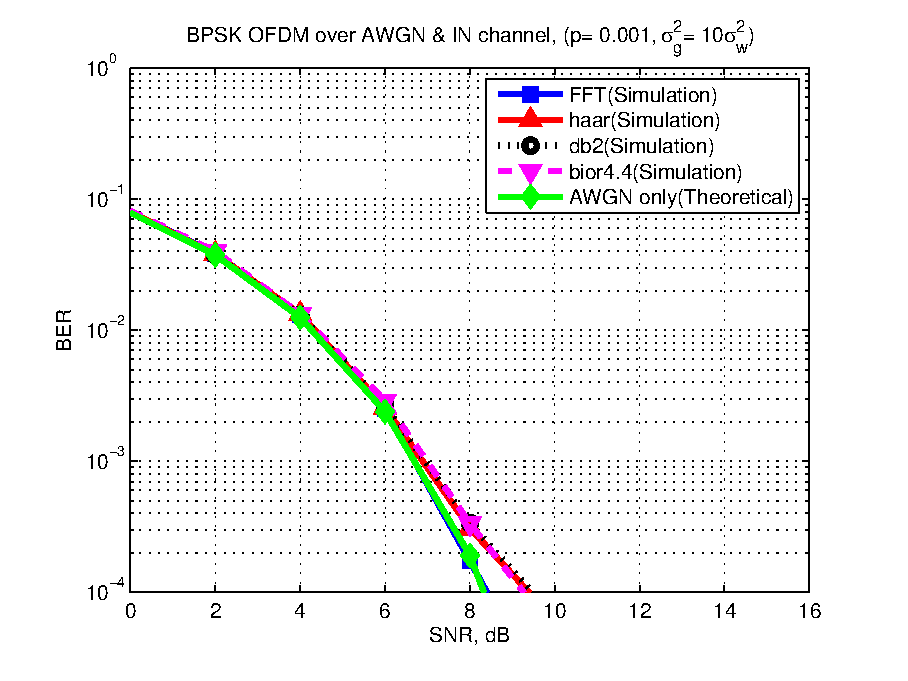
\includegraphics[width=0.6\textwidth]{./chap_4/BPSK_SNR13}}}\\
		\caption{Performance of BPSK OFDM systems in AWGN \& IN ($ \sigma_g^2= 10\sigma_w^2 $ with different values of occurrence probability, $ p $).}
		\label{fig4:BPSK_SNR1}
		\end{figure}

		\begin{figure}[p]
		\centering
		\subfloat[$ p=0.1 $]{\label{subfig4:BPSK_SNR21}{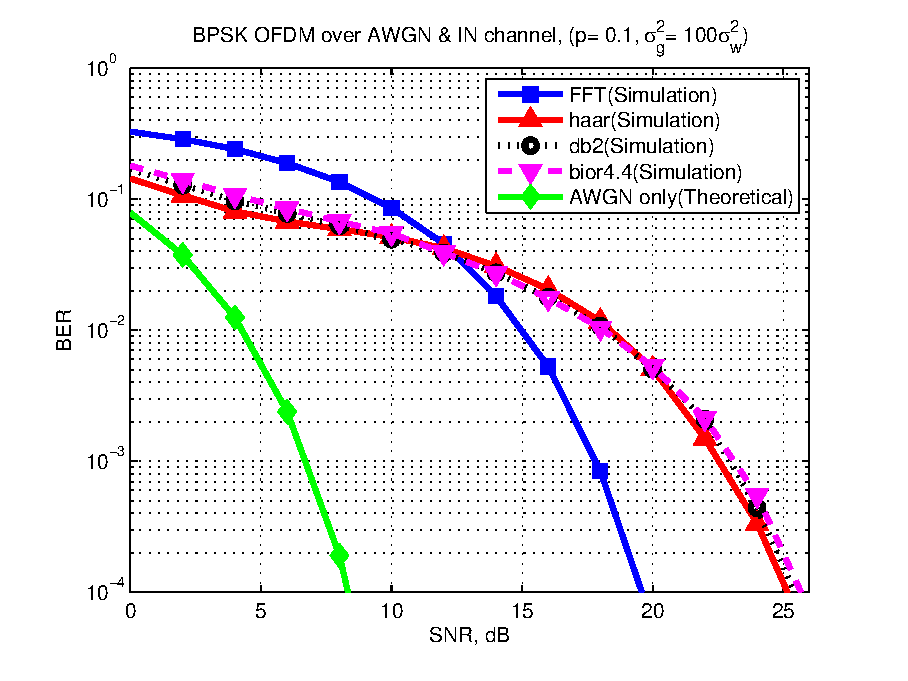
\includegraphics [width=0.6\textwidth]{./chap_4/BPSK_SNR21}}}\\
		\subfloat[$ p=0.01 $]{\label{subfig4:BPSK_SNR22}{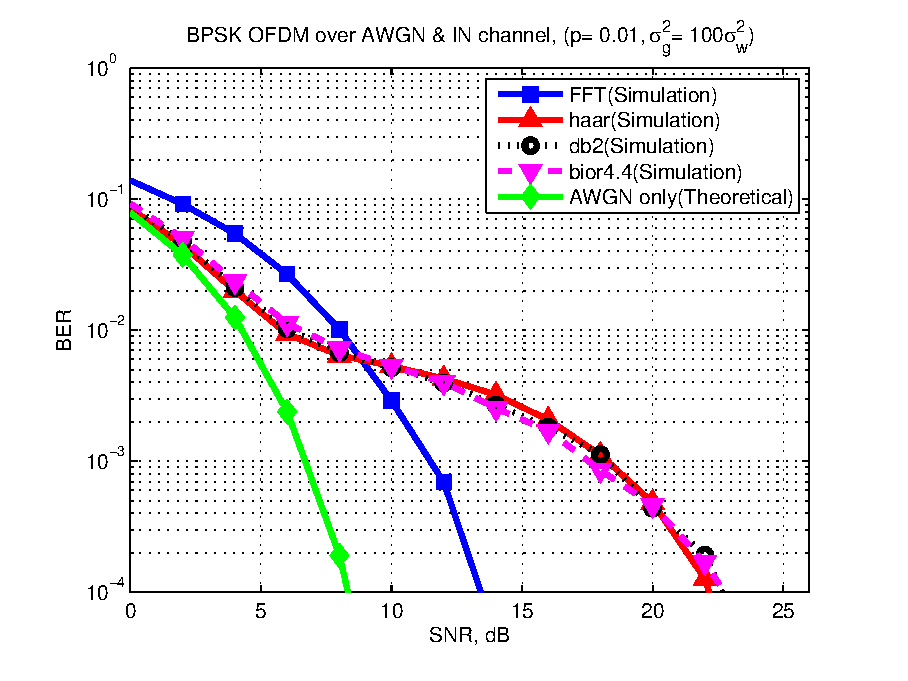
\includegraphics[width=0.6\textwidth]{./chap_4/BPSK_SNR22}}}\\
		\subfloat[$ p=0.001$]{\label{subfig4:BPSK_SNR23}{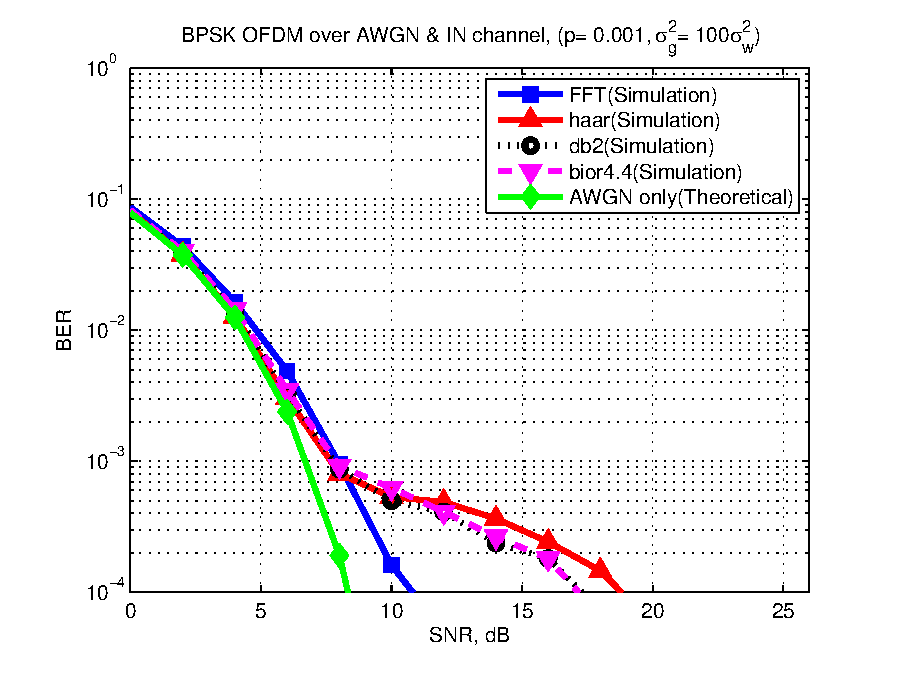
\includegraphics[width=0.6\textwidth]{./chap_4/BPSK_SNR23}}}\\
		\caption{Performance of BPSK OFDM systems in AWGN \& IN ($ \sigma_g^2= 100\sigma_w^2 $ with different values of occurrence probability $ p $).}
		\label{fig4:BPSK_SNR2}
		\end{figure}
		
		\begin{figure}[p]
		\centering
		\subfloat[$ p=0.1 $]{\label{subfig4:BPSK_SNR31}{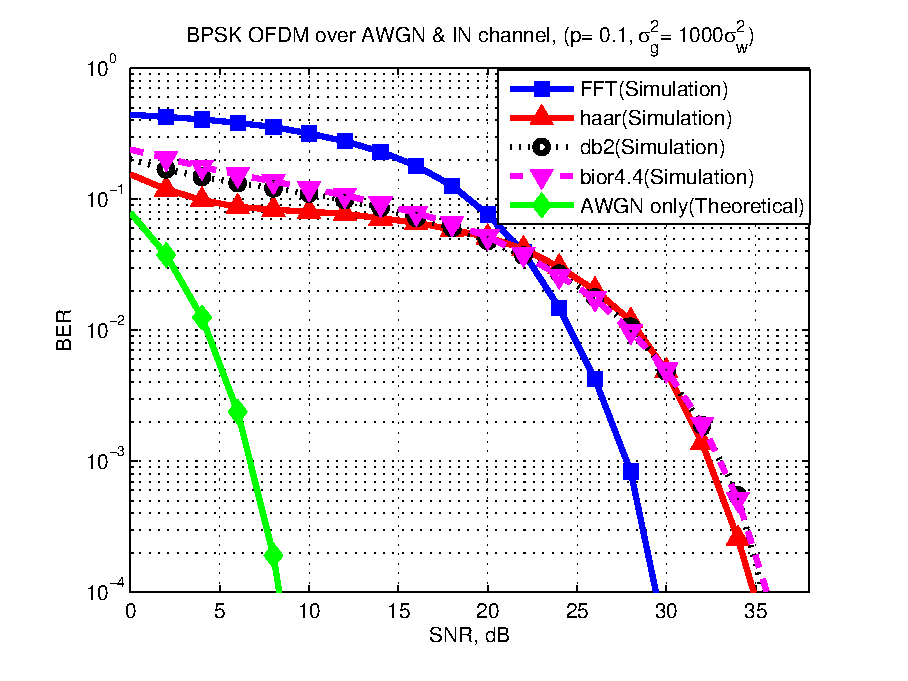
\includegraphics [width=0.6\textwidth]{./chap_4/BPSK_SNR31}}}\\
		\subfloat[$ p=0.01 $]{\label{subfig4:BPSK_SNR32}{\includegraphics[width=0.6\textwidth]{./chap_4/BPSK_SNR32}}}\\
		\subfloat[$ p=0.001$]{\label{subfig4:BPSK_SNR33}{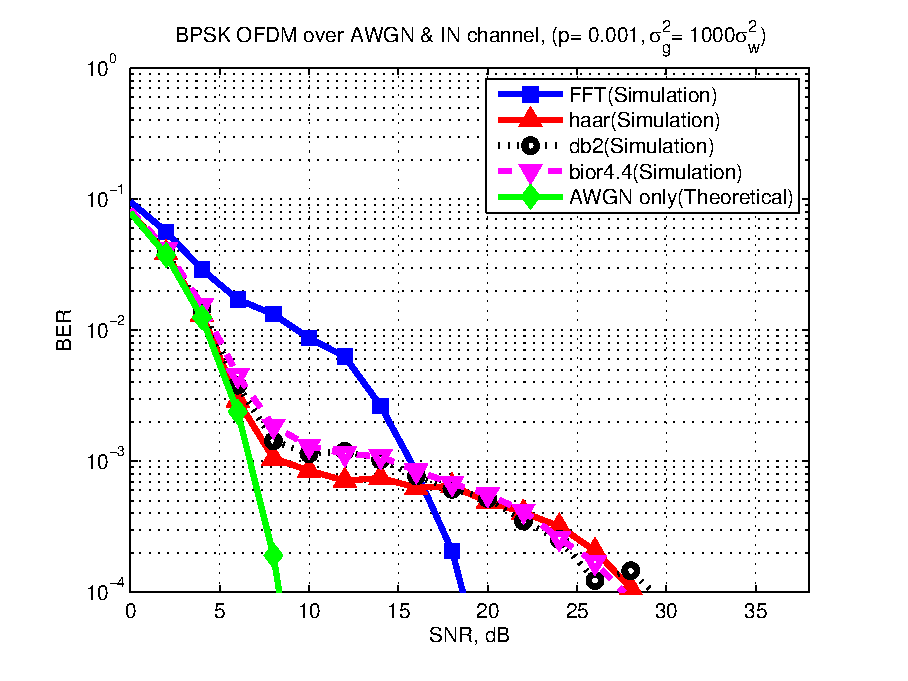
\includegraphics[width=0.6\textwidth]{./chap_4/BPSK_SNR33}}}\\
		\caption{Performance of BPSK OFDM systems in AWGN \& IN ($ \sigma_g^2= 1000\sigma_w^2 $ with different values of occurrence probability, $ p $).}
		\label{fig4:BPSK_SNR3}
		\end{figure}

		\begin{landscape}
			\begin{table}
			\centering
			\caption{BPSK OFDM performance under AWGN \& IN, $\sigma_g^2=f\sigma_w^2 $. }
			\label{tab4:BPSK_SNR}
			\begin{small}
			\begin{tabular}{@{}*9c@{}p{2cm}}
			\toprule[1.5pt]
			&\multirow{3}{*}{$p$} & \multicolumn{3}{c} {\textbf{SNR at BER $ =10^{-4} $}} & \multicolumn{2}{c} {\parbox{3 cm}{\textbf{Same (DWT \& FFT) performance region or point}}} & \multicolumn{2}{c} {\parbox{3 cm}{\textbf{Best DWT performance point (compared to FFT)}}}  \\
			& &  AWGN & DWT & FFT & \multirow{2}{*} {SNR} &  \multirow{2}{*} {BER} & \multirow{2}{*} {SNR} & \multirow{2}{*} {BER$ _{DWT} $} \\
			& & (BER of DWT ) & (BER of FFT) & (BER of DWT)  \\
			\cmidrule(lr){2-2}\cmidrule(lr){3-5}\cmidrule(l){6-7} \cmidrule(l){8-9}
			
			\multirow{6}{*}{$\sigma_g^2=10\sigma_w^2$} &\multirow{2}{*} {$ 0.1 $} & $ 8.5 $ dB & $ 15.8 $ dB & $ 12 $ & \multirow{2}{*}{$= 6$ dB} & \multirow{2}{*}{$3 \times 10^{-2}$}  & \multirow{2}{*}{$= 0$ dB}& \multirow{2}{*}{$1 \times 10^{-1}$} \\
			& & $ 1 \times 10^{-2} $ & - & $3 \times 10^{-3}$ \\
			\cmidrule(lr){3-5}
			
			& \multirow{2}{*} {$ 0.01 $} & $ 8.5 $ dB & $ 13 $ dB & $ 8.8 $ dB & \multirow{2}{*}{$< 2$ dB} & \multirow{2}{*}{$3 \times 10^{-2}$}  & \multirow{2}{*}{-}& \multirow{2}{*}{-} \\
			& & $1.5 \times 10^{-3}$ & - & $1 \times 10^{-3}$ \\
			\cmidrule(lr){3-5}
			
			& \multirow{2}{*} {$ 0.001 $} & $ 8.5 $ dB & $ 9.5 $ dB & $ 8.5 $ dB & \multirow{2}{*}{$< 6$ dB} & \multirow{2}{*}{$1 \times 10^{-3}$}  & \multirow{2}{*}{-}& \multirow{2}{*}{-} \\
			& & $2 \times 10^{-4}$ & - & $2 \times 10^{-4}$ \\
			
			\toprule[1pt]
			
			
			\multirow{6}{*}{$\sigma_g^2=100\sigma_w^2$} &\multirow{2}{*} {$ 0.1 $} & $ 8.5 $ dB & $ 25 $ dB & $ 19 $ & \multirow{2}{*}{$= 12$ dB} & \multirow{2}{*}{$=4 \times 10^{-2}$}  & \multirow{2}{*}{$= 4$ dB}& \multirow{2}{*}{$1 \times 10^{-1}$} \\
			& & $ 6 \times 10^{-2} $ & - & $7 \times 10^{-3}$ \\
			\cmidrule(lr){3-5}
			
			& \multirow{2}{*} {$ 0.01 $} & $ 8.5 $ dB & $ 22.5 $ dB & $ 13.5 $ dB & \multirow{2}{*}{$= 9$ dB} & \multirow{2}{*}{$= 6 \times 10^{-3}$}  & \multirow{2}{*}{-}& \multirow{2}{*}{-} \\
			& & $7 \times 10^{-3}$ & - & $3 \times 10^{-3}$ \\
			\cmidrule(lr){3-5}
			
			& \multirow{2}{*} {$ 0.001 $} & $ 8.5 $ dB & $ 18 $ dB & $ 11 $ dB & \multirow{2}{*}{$< 6$ dB} & \multirow{2}{*}{$1 \times 10^{-3}$}  & \multirow{2}{*}{-}& \multirow{2}{*}{-} \\
			& & $8 \times 10^{-4}$ & - & $5 \times 10^{-4}$ \\
			
			\toprule[1pt]
			
%			
			\multirow{6}{*}{$\sigma_g^2=1000\sigma_w^2$} &\multirow{2}{*} {$ 0.1 $} & $ 8.5 $ dB & $ 35 $ dB & $ 29.5  $ dB & \multirow{2}{*}{$= 22$ dB} & \multirow{2}{*}{$=4\times 10^{-2}$}  & \multirow{2}{*}{$= 4$ dB}& \multirow{2}{*}{$1 \times 10^{-1}$} \\
			& & $ 7 \times 10^{-2} $ & - & $7 \times 10^{-3}$ \\
			\cmidrule(lr){3-5}
			
			& \multirow{2}{*} {$ 0.01 $} & $ 8.5 $ dB & $ 33 $ dB & $ 22.5 $ dB & \multirow{2}{*}{$= 18$ dB} & \multirow{2}{*}{$= 6 \times 10^{-3}$}  & \multirow{2}{*}{-}& \multirow{2}{*}{-} \\
			& & $8 \times 10^{-3}$ & - & $4 \times 10^{-3}$ \\
			\cmidrule(lr){3-5}
			
			& \multirow{2}{*} {$ 0.001 $} & $ 8.5 $ dB & $ 28 $ dB & $ 18.5 $ dB & \multirow{2}{*}{$= 16$ dB} & \multirow{2}{*}{$6 \times 10^{-4}$}  & \multirow{2}{*}{-}& \multirow{2}{*}{-} \\
			& & $8 \times 10^{-4}$ & - & $6 \times 10^{-4}$ \\
			\toprule[1.5pt]
			\end{tabular}
			\end{small}
			%\end{tiny}
			\end{table}
		\end{landscape}


